\documentclass{tufte-book}

\hypersetup{colorlinks}% uncomment this line if you prefer colored hyperlinks (e.g., for onscreen viewing)

%%
% Book metadata
\title{MvdMlab Manual}
%\author[MvdM]{MvdM}
%\publisher{Publisher of This Book}

%%
% If they're installed, use Bergamo and Chantilly from www.fontsite.com.
% They're clones of Bembo and Gill Sans, respectively.
%\IfFileExists{bergamo.sty}{\usepackage[osf]{bergamo}}{}% Bembo
%\IfFileExists{chantill.sty}{\usepackage{chantill}}{}% Gill Sans

%\usepackage{microtype}

%%
% For nicely typeset tabular material
\usepackage{booktabs}

%%
% For graphics / images
\usepackage{graphicx}
\setkeys{Gin}{width=\linewidth,totalheight=\textheight,keepaspectratio}
\graphicspath{{graphics/}}

% The fancyvrb package lets us customize the formatting of verbatim
% environments.  We use a slightly smaller font.
\usepackage{fancyvrb}
\fvset{fontsize=\normalsize}

%%
% Prints argument within hanging parentheses (i.e., parentheses that take
% up no horizontal space).  Useful in tabular environments.
\newcommand{\hangp}[1]{\makebox[0pt][r]{(}#1\makebox[0pt][l]{)}}

%%
% Prints an asterisk that takes up no horizontal space.
% Useful in tabular environments.
\newcommand{\hangstar}{\makebox[0pt][l]{*}}

%%
% Prints a trailing space in a smart way.
\usepackage{xspace}

% Prints the month name (e.g., January) and the year (e.g., 2008)
\newcommand{\monthyear}{%
  \ifcase\month\or January\or February\or March\or April\or May\or June\or
  July\or August\or September\or October\or November\or
  December\fi\space\number\year
}


% Prints an epigraph and speaker in sans serif, all-caps type.
\newcommand{\openepigraph}[2]{%
  %\sffamily\fontsize{14}{16}\selectfont
  \begin{fullwidth}
  \sffamily\large
  \begin{doublespace}
  \noindent\allcaps{#1}\\% epigraph
  \noindent\allcaps{#2}% author
  \end{doublespace}
  \end{fullwidth}
}

% Inserts a blank page
\newcommand{\blankpage}{\newpage\hbox{}\thispagestyle{empty}\newpage}

\usepackage{units}

% Typesets the font size, leading, and measure in the form of 10/12x26 pc.
\newcommand{\measure}[3]{#1/#2$\times$\unit[#3]{pc}}

% Macros for typesetting the documentation
\newcommand{\hlred}[1]{\textcolor{Maroon}{#1}}% prints in red
\newcommand{\hangleft}[1]{\makebox[0pt][r]{#1}}
\newcommand{\hairsp}{\hspace{1pt}}% hair space
\newcommand{\hquad}{\hskip0.5em\relax}% half quad space
\newcommand{\TODO}{\textcolor{red}{\bf TODO!}\xspace}
\newcommand{\ie}{\textit{i.\hairsp{}e.}\xspace}
\newcommand{\eg}{\textit{e.\hairsp{}g.}\xspace}
\newcommand{\na}{\quad--}% used in tables for N/A cells
\providecommand{\XeLaTeX}{X\lower.5ex\hbox{\kern-0.15em\reflectbox{E}}\kern-0.1em\LaTeX}
\newcommand{\tXeLaTeX}{\XeLaTeX\index{XeLaTeX@\protect\XeLaTeX}}
% \index{\texttt{\textbackslash xyz}@\hangleft{\texttt{\textbackslash}}\texttt{xyz}}
\newcommand{\tuftebs}{\symbol{'134}}% a backslash in tt type in OT1/T1
\newcommand{\doccmdnoindex}[2][]{\texttt{\tuftebs#2}}% command name -- adds backslash automatically (and doesn't add cmd to the index)
\newcommand{\doccmddef}[2][]{%
  \hlred{\texttt{\tuftebs#2}}\label{cmd:#2}%
  \ifthenelse{\isempty{#1}}%
    {% add the command to the index
      \index{#2 command@\protect\hangleft{\texttt{\tuftebs}}\texttt{#2}}% command name
    }%
    {% add the command and package to the index
      \index{#2 command@\protect\hangleft{\texttt{\tuftebs}}\texttt{#2} (\texttt{#1} package)}% command name
      \index{#1 package@\texttt{#1} package}\index{packages!#1@\texttt{#1}}% package name
    }%
}% command name -- adds backslash automatically
\newcommand{\doccmd}[2][]{%
  \texttt{\tuftebs#2}%
  \ifthenelse{\isempty{#1}}%
    {% add the command to the index
      \index{#2 command@\protect\hangleft{\texttt{\tuftebs}}\texttt{#2}}% command name
    }%
    {% add the command and package to the index
      \index{#2 command@\protect\hangleft{\texttt{\tuftebs}}\texttt{#2} (\texttt{#1} package)}% command name
      \index{#1 package@\texttt{#1} package}\index{packages!#1@\texttt{#1}}% package name
    }%
}% command name -- adds backslash automatically
\newcommand{\docopt}[1]{\ensuremath{\langle}\textrm{\textit{#1}}\ensuremath{\rangle}}% optional command argument
\newcommand{\docarg}[1]{\textrm{\textit{#1}}}% (required) command argument
\newenvironment{docspec}{\begin{quotation}\ttfamily\parskip0pt\parindent0pt\ignorespaces}{\end{quotation}}% command specification environment
\newcommand{\docenv}[1]{\texttt{#1}\index{#1 environment@\texttt{#1} environment}\index{environments!#1@\texttt{#1}}}% environment name
\newcommand{\docenvdef}[1]{\hlred{\texttt{#1}}\label{env:#1}\index{#1 environment@\texttt{#1} environment}\index{environments!#1@\texttt{#1}}}% environment name
\newcommand{\docpkg}[1]{\texttt{#1}\index{#1 package@\texttt{#1} package}\index{packages!#1@\texttt{#1}}}% package name
\newcommand{\doccls}[1]{\texttt{#1}}% document class name
\newcommand{\docclsopt}[1]{\texttt{#1}\index{#1 class option@\texttt{#1} class option}\index{class options!#1@\texttt{#1}}}% document class option name
\newcommand{\docclsoptdef}[1]{\hlred{\texttt{#1}}\label{clsopt:#1}\index{#1 class option@\texttt{#1} class option}\index{class options!#1@\texttt{#1}}}% document class option name defined
\newcommand{\docmsg}[2]{\bigskip\begin{fullwidth}\noindent\ttfamily#1\end{fullwidth}\medskip\par\noindent#2}
\newcommand{\docfilehook}[2]{\texttt{#1}\index{file hooks!#2}\index{#1@\texttt{#1}}}
\newcommand{\doccounter}[1]{\texttt{#1}\index{#1 counter@\texttt{#1} counter}}

% opening quotes (from https://tex.stackexchange.com/questions/53377/inspirational-quote-at-start-of-chapter)
%\usepackage{epigraph}
\makeatletter
\renewcommand{\@chapapp}{}% Not necessary...
\newenvironment{chapquote}[2][2em]
  {\setlength{\@tempdima}{#1}%
   \def\chapquote@author{#2}%
   \parshape 1 \@tempdima \dimexpr\textwidth-2\@tempdima\relax%
   \itshape}
  {\par\normalfont\hfill--\ \chapquote@author\hspace*{\@tempdima}\par\bigskip}
\makeatother

% Generates the index
\usepackage{makeidx}
\makeindex

\usepackage{color}
\definecolor{lightgray}{gray}{0.75}

\newcommand\greybox[1]{%
  \vskip\baselineskip%
  \par\noindent\colorbox{lightgray}{%
    \begin{minipage}{\textwidth}#1\end{minipage}%
  }%
  \vskip\baselineskip%
}

\usepackage[parfill]{parskip}
\setlength{\parindent}{0pt} % hmm neither of these options get rid of
                            % the indent! -- MvdM

\begin{document}

% Front matter
%\frontmatter

% r.1 blank page
%\blankpage

% v.2 epigraphs
%\newpage\thispagestyle{empty}
%\openepigraph{%
%A designer knows that he has achieved perfection 
%not when there is nothing left to add, 
%but when there is nothing left to take away.
%}{Antoine de Saint-Exup\'{e}ry}
%\vfill

% r.3 full title page
\maketitle

% r. 4 copyright and attributions
\newpage
\begin{fullwidth}
~\vfill
\thispagestyle{empty}
\setlength{\parindent}{0pt}
\setlength{\parskip}{\baselineskip}
Copyright \copyright\ \the\year\ van der Meer lab

\par\smallcaps{www.vandermeerlab.org}

\begin{figure}
  
\includegraphics[width=5cm]{images/license.png}
%  \checkparity This is an \pageparity\ page.%
\end{figure}


\par Licensed under the Creative Commons BY-NC-SA License (the
``License''), version 4.0; you may not use this file except in
compliance with the License. Briefly, you are free to share and adapt
this material, under the condition that you give appropriate credit,
do not use the material for commercial purposes, and distribute your
contributions under the same terms. You may obtain a copy of the full
License at \url{https://creativecommons.org/licenses/by-nc-sa/4.0/}.

\par Inspired by similar lab manuals by others. Particularly helpful
were the wonderful examples from the
\href{http://jpeelle.net/peellelab_manual.pdf}{Peelle} and \href{https://github.com/alylab/labmanual}{Aly} labs.

\par Typeset in Palatino Linotype using \LaTeX{} and the
\doccls{tufte-book} class.

\par\textit{Version 0.3, \monthyear}
\end{fullwidth}

% r.4 contents
\setcounter{tocdepth}{1}
\tableofcontents

% r.9 introduction
\chapter{Welcome!}

\newthought{The van der Meer lab} brings together people who share an
interest in how the brain works. We aim to better understand how
learning, memory, and decision-making arise from the coordinated
activity of neurons. In the pursuit of this goal, we perform brain
surgery, design and construct eclectic mazes, painstakingly build
small devices so we can read the minds of rats, solder tiny circuit
boards to even tinier wires, write thousands of lines of computer
code, collect beautiful data, produce even more beautiful plots, and
wonder what it all means.

\begin{marginfigure}[-4cm]
\centering{
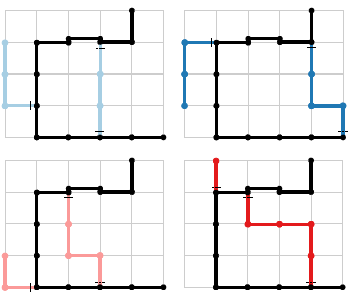
\includegraphics[width=0.7\linewidth]{images/shortcut_mazes.png}
}
\caption{Example maze configurations. (From Emily Irvine's {\it
    shortcut} experiment.)}
\label{fig:shortcut}
\end{marginfigure}

\newthought{Each of us brings} their own particular blend of
motivations for engaging in these lab activities, but there are a few
common threads: curiosity about how the physical stuff of the brain
gives rise to thought and to behavior, a love for animals and
computers\sidenote{Or, at least, a love of computable things.}
alike, a desire to help solve some of the big mysteries, and
contributing to human knowledge and ultimately a better world.

\begin{marginfigure}[3cm]
\centering{
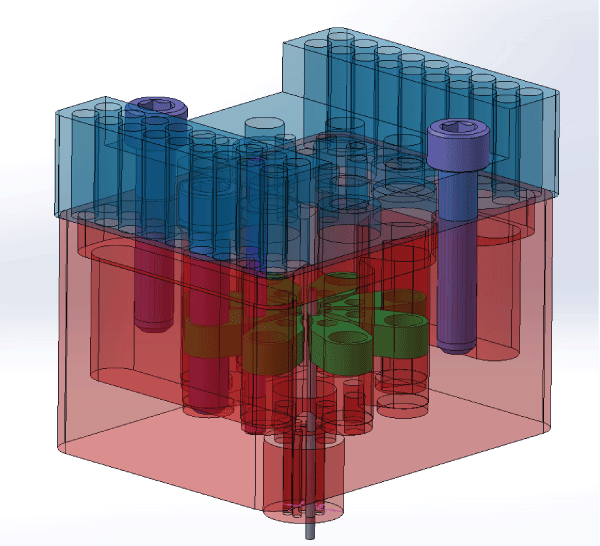
\includegraphics[width=0.7\linewidth]{images/8tt_drive.png}
}
\caption{A small device for rat mind-reading (by Andrew Alvarenga).}
\label{fig:8tt_drive}
\end{marginfigure}

\newthought{Our efforts are {\it collaborative}}, not only within the
lab, but also with other labs in the department of Psychological \&
Brain Sciences at Dartmouth. We share equipment, space, and interests
with these labs, and collaborate not only on joint scientific
projects, but also on creating a scientifically exciting and
supportive culture where everyone can thrive. We also have joint
projects with other labs around the world. We collaborate because the
problems we are trying to solve are hard, and because learning from
and working with others is one of the great joys of working in
science!

\newthought{Working with others} brings not only joy, but also
expectations. Coding and data analysis can be fun, but are full of
pitfalls. Sharing space and expensive equipment with others demands
care and respect. There is satisfaction in getting an experiment to
work, but it can be a long slog to get there. Perhaps most importantly
of all, the use of animals in research comes with practical as well as
moral responsibilities. {\it This manual is intended to provide
  guidance on how to navigate these issues, with particular focus on
  the van der Meer lab.}

\begin{marginfigure}
\centering{
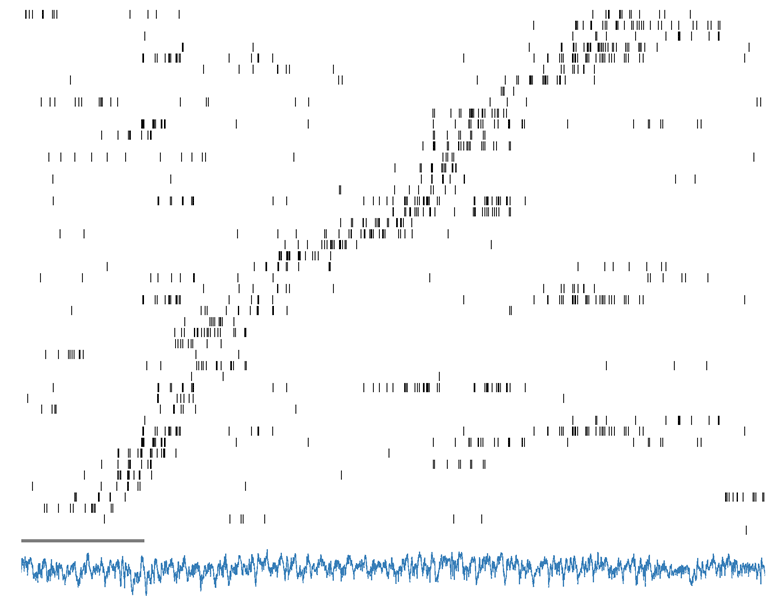
\includegraphics[width=\linewidth]{images/R050_raster.png}
}
\caption{Some beautiful data, recorded from R050's hippocampus (by
  Alyssa Carey). Vertical tick marks indicate spikes (one row per
  neuron, sorted by place field location); horizontal axis indicates
  time; blue trace shows a local field potential. Scale bar is 1 s.}
\label{fig:raster}
\end{marginfigure}

\newthought{If you are new to the lab}, I would like you to read this
manual through in its entirety. If you will not be working with
animals directly, it may seem like chapter on
\hyperref[sec:animal-management]{Animal Management} does not apply to
you, but it will give you important insights into how the lab
operates.

\newthought{Welcome}. Let's do some great science together!

\begin{chapquote}{{\it MvdM}}
\end{chapquote}
%%
% Start the main matter (normal chapters)
\mainmatter

\chapter{About this manual}

\newthought{This document} describes the principles that shape how the
members of the lab interact and work. Rather than dealing with the
nuts and bolts of how to get stuff done in the lab, the manual is
about lab philosophy, expectations, and resources. It is an
introduction to the lab. The lab manual is one of several classes
(categories) of shared documents in the lab, which are:

\begin{itemize}
\item{{\it Lab Manual}. You are looking at it. It contains information
  that does not change frequently. Only MvdM can change the lab
  manual, but I'd love to hear from you if you have thoughts of
  suggestions! Periodically, we may review the manual as a group at
  lab meeting to determine what needs updating.}
\item{Private {\it GitHub
    repositories}\sidenote{\url{www.github.com/vandermeerlab}. Because
    these repositories are private, you will not be able to see them
    unless you are logged in and a member of the vandermeerlab
    organization.} that contain \doccls{protocols},
  i.e.\ documentation for experimental procedures\sidenote{Examples
    include electrode plating, histology, drive building, et cetera:
    see the \url{mvdmlab-protocols} repository}, and a separate repository for
  \doccls{behavioral tasks} and associated computer
  code\sidenote{\url{mvdmlab-tasks}}. This documentation is on GitHub
  so that we can say things like, ``I used version 1.1 of the
  histology protocol'', and so that we can track changes to those
  protocols as well as the reasons for those changes. If you perform
  procedures in the lab, you are expected to follow and to contribute
  to these protocols; see the \href{sec:notes}{Documentation} section for
  more detailed information.}
\item{A {\it lab
    wiki}\sidenote{\url{rcweb.dartmouth.edu/~mvdm/wiki}} that
  contains tutorials, guides, lists of useful links, et cetera. The
  wiki is a more dynamic, easier to edit resource for content that
  doesn't rely as much on version control. The wiki currently contains
  the lab's MATLAB data analysis tutorials.}
\item{We also have a lab {\it Slack}
  team\sidenote{\url{mvdmlab.slack.com}. If you are new to the lab and
    you haven't received an invitation email to join it, e-mail MvdM.}
  which is used for day to day communication. It hosts shared
  documents best described as ``everything else'', something that
  isn't a protocol, task, or tutorial.}
\end{itemize}

These different venues reflect an overall organization ranging from
content that is easy to create and easy to change (low overhead,
quick; Slack, wiki), to content that is moderately stable and takes a
bit more effort to change (but easier to track; GitHub), to principles
that rarely change (lab manual). For instance, an idea for an
experiment may be initially discussed on Slack, lead to a draft
protocol shared there, and then get pushed to GitHub. 

There are a number of other kinds of documents used in the lab that,
unlike the above categories, are not typically consulted by multiple
lab members. Most important among these are (1) animal records,
described in more detail in the \hyperref[ch:animal-management]{Animal
  Recordkeeping} chapter, and (2) lab notebooks/notes, described in
the \hyperref[sec:notes]{Keeping Good Notes} section.

\greybox{
\textsf{\textbf{Important:} I assume the lab manual and procedures on GitHub are
  accurate. This means that you should follow all of the policies and
  procedures contained in the manual and GitHub. If you notice
  something that seems to be wrong, please let me know (for the lab
  manual) or change it yourself (if on GitHub). If there is something in
  the lab manual or GitHub that you notice people aren't doing, please
  bring this up at lab meeting, or to me directly. Don't assume this
  is okay (it's not).}}

%%% RESEARCH USING ANIMALS &&&
\chapter{Research Using Animals}
\label{ch:animals}

\newthought{We use animals} in the lab, based on the conviction that
doing so accelerates scientific progess and provides a net benefit to
humans, and perhaps to animals, too. There are many examples of
scientific discoveries that were directly enabled by research in
animals\sidenote{Some good examples are highlighted in the ``Position
  statement of the Max Planck Society concerning the use of animals in
  experiments for basic research''
  (\href{https://www.mpg.de/10882259/MPG_Whitepaper.pdf}{link})}. However,
past successes do not mean we can experiment freely on any animal we
want. The use of animals for research carries a moral, scientific, and
legal obligation to only perform experiments when the benefits can be
reasonably expected to outweigh the costs, to do so only if no
suitable alternatives are available, and to do so while caring for our
animals to the fullest extent possible. These notions are often
phrased as the ``3 R's'' (reduction, replacement,
refinement)\sidenote{Good references on this topic include
  \href{https://www.nc3rs.org.uk/the-3rs}{NC3Rs}.}.

\begin{marginfigure}
\centering{
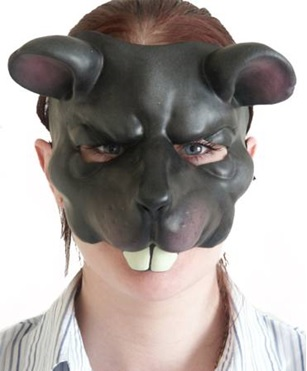
\includegraphics[width=0.7\linewidth]{images/rat-mask.jpg}
}
\caption{A visual allegory for synergy between humans and rats.}
\label{fig:rat-mask}
\end{marginfigure}

More generally, research in animals demands that we do the best job
possible, and maximize the usefulness of the research outcomes.

This means that:

\begin{itemize}

\item{{\it We take care of our animals}. If animals are comfortable and well
  cared for, they will perform the behavioral tasks we want, be easier
  to handle, and the resulting fundings will be more likely to generalize.}

\item{We strive to {\it design experiments such that the outcomes will
    be as informative as possible}. There are many resources on this
  topic, including the specific demands on rigor and reproducibility
  mandated by the NIH
  (\href{https://grants.nih.gov/policy/reproducibility/index.htm}{link}). Many
  experimental design decisions can be brought into focus by perparing
  a formal \href{https://cos.io/prereg/}{preregistration} of your
  proposed experiment, which requires justifying how many subjects you
  plan to run, what analyses you will carry out, and the inferences
  supported by possible outcomes.}

\item{We aim to collect the {\it highest quality data possible}. We
  often invest a tremendous amount of time in each animal through
  behavioral training, construction of chronic implants, surgery, and
  so on. If any one of these procedures is not performed diligently,
  then your investment in all the others may come to nothing.}

\item{For the data to be interpretable, {\it good records} need to be
  kept. Recordkeeping includes informal written notes and the
  completion of highly organized templates produced as procedures are
  performed. Good recordkeeping also encompasses the process of
  translating these notes into computer-readable formats suitable for
  data analysis.}

\item{{\it Data is valuable}. It needs to be protected against inadvertent
  loss, and its impact needs to be maximized by making it possible for
  a single data set to inform multiple questions, including those
  asked by different investigators within and outside the lab. This
  means it needs to be organized and annotated in a specific common
  format.}
\end{itemize}

In sum, the fact we are working with animals shapes both our lab
philosophy and many practical aspects of working in the lab. Much of
the content that follows in this manual is essentially unpacking the
above points in more detail.

\begin{marginfigure}
\centering{
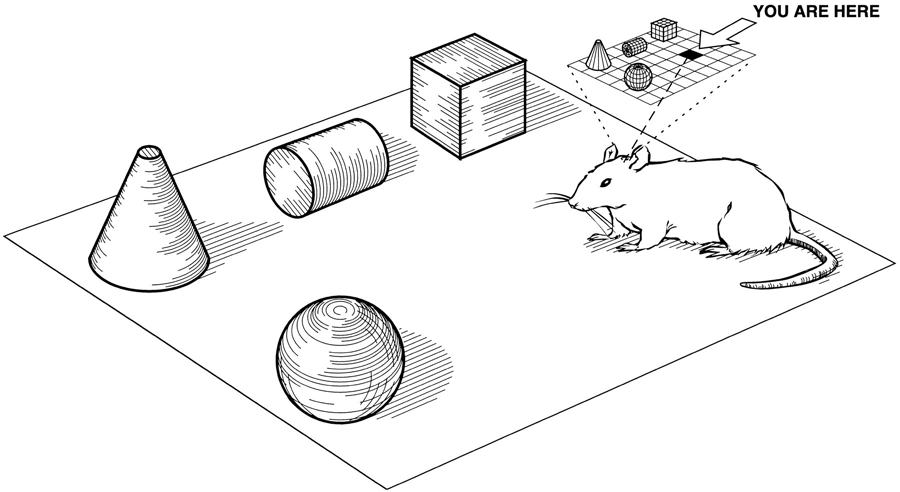
\includegraphics[width=0.9\linewidth]{images/rat_with_objects.png}
}
\caption{A cartoon rat with some objects (from
  \citealt{Eichenbaum1999a}).}
\label{fig:rat-with-objects}
\end{marginfigure}

\newthought{Animal research at Dartmouth} is overseen by the
Institutional Animal Care and Use Committee (IACUC). All work with
animals needs to receive prior approval from the IACUC in the form of
{\it Animal Use Protocols} (AUPs) \sidenote{{\it Animal Use Protocol}:
  document outlining the scientific rationale, aims, and a set of
  proposed experiments, including specific animal numbers for
  each. The total number of approved animals may not be
  exceeded.}. Only {\it procedures}\sidenote{{\it Procedure:} Any
  action or change beyond picking an animal up in the colony room
  (e.g.\ for changing cages or weighing) counts as a procedure. This
  includes, among others, placing an animal on a restricted diet,
  running a behavioral task, and injecting an analgesic.} that have
been approved by the IACUC may be performed on animals, and only by
approved personnel (listed on the protocol). We are {\bf required} to
log all procedures; details on this process can be found in the
\hyperref[ch:animal-management]{Animal recordkeeping}
chapter. Invasive procedures, such as electrode implant surgery,
require follow-up procedures providing post-operative care
(administration of analgesia, monitoring).

To be formally approved to perform any of the procedures described in
an AUP, a number of on-line and in-person training modules need to be
completed. To initiate the training process, e-mail MvdM, and please
forward copies of any confirmation of training completion. The current
version of all AUPs can be found in the \url{#animalcareandrecords}
channel on the \href{http://mvdmlab.slack.com}{lab Slack}.

\greybox{ \textsf{\textbf{Important}: Violations of the above
    requirements, such as performing a procedure not previously
    approved, or neglecting to log a procedure that was performed, are
    serious. Beyond potentially violating our moral responsibility
    towards our animal subjects, the lab, the department, and
    Dartmouth risks losing federal approval to perform animal research
    if found delinquent. Systems are in place to minimize the
    likelihood of mistakes from happening; however, we are all human
    and mistakes do happen. If you notice any slips, please take
    action: rectify if you can, consider how to prevent this happening
    again, and let MvdM know. Transparency and honesty about what
    occurred is always the best course of action.}}


%%%%%%%%%%%%%%%%%%%%
%%% ANIMAL CARE %%%%
%%%%%%%%%%%%%%%%%%%%
\section{Animal care and recordkeeping}
\label{sec:animalcare}

\newthought{Keeping detailed and accurate records} on each of our
animals is an IACUC requirement (and indirectly a federal issue), as
well as scientifically important. The main principles are that for any
animal that is currently alive, there must a binder (or a section in a
binder) with that animal that contains an up to date record of all
procedures\sidenote{What counts as a procedure: anything beyond what's
  required to change a cage or weigh an animal. If in doubt, log it
  anyway.} performed on that animal, as well as records of their
weight.

\newthought{Animal husbandry\sidenote{That is, animal care not
    consisting of procedures, such as changing cages and providing
    food and water.} at Dartmouth} is provided by the Center for
Comparative Medicine Research (CCMR). CCMR maintains a satellite
animal facility in the basement of Moore Hall, where our animals are
housed and cared for by CCMR staff. CCMR also employs veterinary
staff, who are ``on call'' to provide support and advice (and in
unusual cases, can mandate an animal be euthanized). Up-to-date
contact information for CCMR staff and vets can be found in the
\url{#animalcareandrecords} channel. When performing invasive
procedures (surgery) and when administering drugs, CCMR requests that
these are reported using a special cage card\sidenote{Picture of
  procedure cage card.}. Writing procedures on these cards is {\it
  not} sufficient logging: you also need to log the procedure(s) in
the animal's binder.

By default, CCMR staff will feed, water, and change cages for all our
animals. We pay them a {\it per diem} fee to do this. Unless requested
otherwise, all animals receive {\it ad lib}\sidenote{Ad libitem is the
  Latin phrase for, literally, ``to your libido'', i.e.\ as much as
  desired. Incidentally, {\it i.e.}\ is Latin for {\it id est}, ``it
  is''.} food and water.

We can also request CCMR to feed rats 18g/day. This is a useful amount
that prevents rats from getting obese. To request this, use the
relevant cage card\sidenote{This one.}. For any other food/water
regimens, you'll need to use the ``Experimenter will feed/water'' cage
card. Doing so implies that the experimenter listed takes
\doccls{ownership}\sidenote{As the owner of an animal, you are
  responsible for logging its weight and all procedures. If the animal
  is food and/or water-restricted, you are responsible for supplying
  those things, and logging that you have done so.} of that animal.

When animals first arrive, they are typically group-housed (multiple
animals per cage). They are named\sidenote{Rats are named Rxxx, where
  xxx is a 3-digit counter that it incremented with each new
  animal. Mice are named Mxxx.} and start out with \doccls{communal}
status. Communal animals do not have an owner yet. They are weighed
weekly by the \doccls{Communal Animal Caretaker}\sidenote{Note that to
  track weights of group-housed animals, some kind of mark needs to be
  used. The lab convention is to write numbers 1, 2, 3 etc.\ on the
  base of the tail with a Sharpie. 1 indicates the animal with the
  lowest number. Mouse tails are too small to write numbers; stripes
  or rings can be used instead.}. When communal animals are below 400g
in weight, the Caretaker also handles them weekly (about 5 minutes per
animal appears to be the sweet spot, although you may want to take
ownership of an animal that will be implanted with a hyperdrive early
on so that it can be handled more). When communal animals reach 400g,
the Caretaker separates them into individual cages so that CCMR can
feed them 18g/day.

Once you euthanize and animal (or request it to be euthanized),
collect all weight and procedure logs, along with any additional
information (notes from behavior, for instance), scan them into a
single PDF\sidenote{The departmental copier/scanner is great for this,
  you can feed it a pile of documents and it can email you a PDF.} and
upload to the data vault (see the section on Promoting Data).

If you are working with animals, read the \href{github link}{Animal
  Recordkeeping Protocol}, which provides detailed procedures for the
above.

%%%%%%%%%%%%%%%%%%%%
%%% EXPECTATIONS %%%
%%%%%%%%%%%%%%%%%%%%

\chapter{Values and Expectations}\label{ch:expectations}

\newthought{The lab values} personal and scientific integrity, respect
for each other, for animals, for equipment, and for data. We care
about shaping and maintaining an environment that fosters personal
development, curiosity, exploration, and the joy of discovery. We
choose to work on hard problems that require dedication, persistence,
resourcefulness, resilience, and humility. We support each other in
when things get tough, and celebrate each other's successes. We value
opportunities to learn from each other, set high standards but do not
judge.

\newthought{Holding these values} implies the following:

\section{Code of Conduct}

\newthought{The lab is committed} to providing a safe, friendly, and
accepting environment for everybody. We will not tolerate any verbal
or physical harassment or discrimination on the basis of gender,
gender identity and expression, sexual orientation, disability,
physical appearance, body size, country of origin, native language,
race, or religion. We will not tolerate intimidation, stalking,
following, unwanted photography or video recording, sustained
disruption of talks or other events, inappropriate physical contact,
and unwelcome sexual attention. To my knowledge, none of these have
ever occurred in the lab -- let's keep it that way.

Nevertheless, if you notice or experience any of these, please tell
MvdM. If you have an issue with a member of the lab, tell MvdM. If you
have an issue with MvdM that you are not comfortable discussing, the
graduate student representative, department chair, and other faculty
are available, as well as the resources listed below. Please be
assured that your concerns will be taken seriously, that you will be
listened to, and that you can share them without fear of
retaliation. Note the distinction between {\it private resources} and
{\it confidential resources}\sidenote{Private resources are legally
  obligated to share a disclosure of sexual misconduct with the Title
  IX office, including all details that are known. This is to ensure
  adequate support for those who may need it. Confidential resources
  may not share any information (with very few exceptions).}.

Before taking pictures or videos with a lab member in them, ask their
consent first. Ask consent again before posting to social media. If
you'd like to take pictures or videos of an experimental subject, ask
permission from MvdM first.

\newthought{Important resources}:

\begin{itemize}
\item{Dartmouth policies: \href{https://student-affairs.dartmouth.edu/policy/standards-conduct}{undergraduate} and \href{https://graduate.dartmouth.edu/policy/code-conduct-nonacademic-regulations}{graduate} code of conduct}
\item{PBS \href{https://pbs.dartmouth.edu/diversity}{diversity page}.}
\item{Confidential resources on campus:
  \href{http://www.wiseuv.org/dartmouth---home.html}{WISE}\sidenote{A
    WISE advocate is on campus one day a week; see the website for
    details.},
  \href{https://students.dartmouth.edu/health-service/counseling/about/clinical-services/counseling}{counselors}
  at Dick's House, religious leaders at the
  \href{https://students.dartmouth.edu/tucker/about/pastoral-counseling}{Tucker
    Center}}
\item{Private resources: MvdM, PBS department chair, PBS graduate
  chair, other faculty you trust}
\item{Dartmouth \href{https://journeys.dartmouth.edu/knowyourrights/resources/}{Title IX resources}}
\end{itemize}

\section{Expectations: everyone}

\newthought{Big picture:}

\begin{itemize}
\item{{\it Community}. Behave respectfully and professionally towards
  others in the lab, department, and beyond. Doing this well requires
  considering how your actions (or lack of them) affect
  others\sidenote{See the
    \href{https://www.recurse.com/code-of-conduct}{Recurse guidelines}
    for some great examples.}. We value behaviors that enable everyone
  to flourish, and that recognize that in academia, it's easy to feel
  like you don't know enough or aren't doing enough. Build each other
  up, instead of making others feel like they don't belong.}
\item{{\it Collaborate}. Share your expertise. Make arrangements with others
  to take care of their animals one weekend and reciprocate
  another. Offer to do code reviews, read each other's manuscript,
  offer feedback on practive talks.}
\item{{\it Contribute} to community resources and space. If you notice
  something that can be improved, fix it, mention it on Slack, or open
  a GitHub issue.}
\item{{\it Communicate}. Tell others what you are working on, what is
  working well and what could be improved. Post updates on Slack
  frequently -- sharing when you are stuck and what you have tried
  to get unstuck is just as important as sharing successes.}
\item{Take care of yourself. Know when it's time to push, and when
  it's time to take a walk in Pine Park\sidenote{See
    \href{https://www.hanovernh.org/conservation-commission/pages/trail-maps}{here}
    for a guide to some of Hanover's best trails, accessible from the
    lab in the space of a lunch break.}.}
\item{Tell others when you notice they did something well, or when
  they made your life a little better today\sidenote{We have the
    \doccls{octothorp}, awarded during lab meeting. But don't stop
    there!}.}
\item{Be a little obsessive, and have high standards.}
\item{Show up and keep at it. While brilliant ideas, creativity and skill
  certainly help, the best predictor of success is how consistently
  you put in the work. There will be days when it feels like you aren't
  making any progress and nothing is working. Don't underestimate the
  power of an iterative routine}
\end{itemize}

\newthought{Small picture}:

\begin{itemize}
\item{Document. Anything you do more than once, or that you or someone
  else might have to do again, should be written up as a
  \doccls{experimental protocol}\sidenote{Not to be confused with an
    animal (IACUC) protocol.}. Anything done with an animal is a
  \doccls{procedure} and needs to be logged. Good recordkeeping is
  essential to doing good science. Keep track of what you did with
  experiments and analyses in your \doccls{lab notebook}.}
\item{Treat your animal subjects with care, as laid out in the
  \href{ch:animals}{Research with Animals} section.}
\item{Participate in our weekly lab meetings.}
\item{Be punctual and consistent if you are running experiments. Hours
  can be somewhat flexible, but in general all full-time lab members
  are expected to be in at work during at least the core hours of
  11-4, so that we can interact. If you are going to be away from the
  lab for more than a day or two, enter it into the lab calendar.}
\item{If you purchase anything with a \doccls{chart string}\sidenote{A
    Dartmouth-internal number that allows expenses to be charged to
    the correct account and category.}, take a picture of the receipt
  and post it in the \#admin channel on Slack.}
\end{itemize}

% pi
\section{Principal Investigator}

\newthought{I promise to:}

\begin{itemize}
\item{Provide an environment where great science can be done and
  people can thrive.}
\item{Model the different aspects of the scientific process and
  different components of an academic career.}
\item{Give my perspective on
  where the field is going, and how work in the lab will help shape
  that direction.}
\item{Secure operating funds for the lab, which may include your
  stipend or salary.}
\item{Be a mentor, supporter, and resource for you. This includes
  providing you with training in diverse aspects of science, helping
  you set priorities in the short and long term, promote your work and
  helping you identify opportunities.}
\item{Set high standards and commit the time to help you meet them. In
  particular, I will hold weekly lab meetings and project one-on-ones
  with you. I will also give you timely feedback on project ideas,
  conference posters, talks, manuscripts, figures, grants.}
\item{Support and monitor your trajectory in yearly feedback
  meetings.}
\end{itemize}

\section{Graduate Students}\label{sec:gradstudents}

\begin{itemize}
\item{By the time you graduate, you are expected to make an original
  contribution to knowledge, in the form of a thesis that you will
  defend.} 
\item{In the process of reaching this goal, you will build a portfolio
  of published work as well as a set of skills. Become really good at
  at least one marketable technique or skill.}
\item{When you first join the lab, you are expected to take on an existing
or previously proposed project, so you can learn the ropes with plenty
of interaction time with MvdM and senior lab members. As you progress,
you are expected to take a more active role in helping to shape
project directions within the scope of the lab's current and planned
funding.}
\item{Your productivity is expected to be low initially (1-2 years), but
then ramp up. Expect to submit at least one paper per year in years
3+. Research is the clear priority -- avoid spending too much time on
coursework and teaching assistantships.}
\item{Become the world expert on your thesis topic. Read superficially
  in a broad area, and deep in your chosen area\sidenote{See ``How to
    read a book'' book and MvdM's slides for some pointers on
    different kinds of reading. Keep abreast of current developments
    by signing up for key journal table of contents, and use
    crowdsourcing for recommendations (e.g.\ Twitter).}.}
\item{Submit fellowship applications. Help MvdM write grants and review
papers.}
\item{Be aware of the program requirements, and everything else that is in
the PBS grad guide.  Be in charge of these program
requirements. Coursework and milestones.}
\item{Attend B4, and present regularly (this is a program
  requirement). Attend lab journal clubs, and take initiative in
  proposing a journal club topic or paper from time to time.}
\item{Attend departmental colloquia, and go to lunch with the speaker a few
times each year.}
\item{Participate in Dartmouth research events (Neuroscience Day),
  regional meetings, and major conferences in the field such as the
  Society for Neuroscience annual meeting\sidenote{Note that you need
    to be a student member to attend; see \url{www.sfn.org} for
    info.}, \href{www.cosyne.org}{CoSyNe}, Biological Psychiatry, or
  others.}
\item{Participate in rotating lab assignments that change on a term-by-term
basis (animal care, space, codebase, protocols, journal club chair,
social chair).}
\item{Attend a summer school such as Neural Systems \& Behavior at
  MBL\sidenote{\url{www.mbl.edu/nsb}; Eric and Alyssa have TAd at it,
    MvdM and Youki were students, and MvdM has taught there for
    several years.}, the Okinawa Computational Neuroscience
  Course\sidenote{Eric was a student, and MvdM has TAd at it.}, and
  others.}
\item{Be aware of what is required to take the next step of career
  paths you are considering\sidenote{A great starting points for
    thinking about industry vs.\ academia is
    \href{https://www.amazon.com/Navigating-Path-Industry-Managers-Academics-ebook/dp/B00NABNFVW}{this
      book}; lab alumni are also a great resource.}. If you are
  thinking about postdocs, identify potential advisors early on and
  take steps to get them to know about you and your work. Read some
  example letters of recommendation, and proactively consider what you
  would like yours to say.}
\item{If you are going to be away from the lab for more than a day or
  two, let MvdM know and enter the dates in the \href{ADD LAB CALENDAR
    LINK}{lab calendar}.}
\item{Take an active role in monitoring and promoting your mental
  health\sidenote{Some starting points for online resources include
    \href{https://www.gograd.org/resources/grad-student-mental-health/}{GoGrad},
    Dartmouth's graduate school
    \href{https://graduate.dartmouth.edu/academics/academic-calendar/grad-mental-health-awareness-month-2018}{Mental
      Health Awareness program} and
    \href{https://graduate.dartmouth.edu/about/life-community/student-services/health-wellness}{Health
      \& Wellness resource list}.}.}
\item{Don't forget that this is a special time in your life where you get
  to immerse yourself in a topic you are passionate about.}
\end{itemize}

% techs
\section{Research Technicians}

\begin{itemize}
\item{Model good lab practices such as recordkeeping, labeling, and
  organization of lab spaces.}
\item{Work regular hours as defined by your contract. Flexibility is
encouraged, but seek approval from MvdM first.}
\item{cc MvdM on all PCARD transactions when you send them to the
  departmental administrator for reconciliation. Request permission
  first for anything unusual and anything over \$500.}
\item{Discuss attending talks (B4, departmental colloquia) with MvdM
  first before going.}
\end{itemize}

% ugrad
\section{Undergraduates}

\begin{itemize}
\item{Participating in research is different from taking a
  class. Coursework typically consists of specific assignments with
  instructions which you can follow. Research typically centers on a
  question or objective, and you will need to figure out how to make
  progress with it. Take an active role in identifying how to measure
  that progress, and how to tell when you are stuck. If you are stuck,
  discuss possible solutions on Slack and/or with other lab members.}
\item{Especially if you do animal work, reliability and punctuality is
  crucial. Be realistic about the time you can commit when you have to
  balance exams and other activities, and plan ahead.}
\item{Letters of recommendation. You can expect me to write letters of
  recommendation for you if you have worked in the lab for a year
  (three terms) or more\sidenote{When requesting letters of
    recommendation, please allow sufficient time (at least two
    weeks). If you are applying to multiple programs, provide a single
    document, such as a spreadsheet, listing the key information for
    each. When requesting letters, attach your personal statement, CV,
    and specific details you would like to be highlighted in the
    letter. Send a reminder email a few days before each deadline if
    you haven't yet received confirmation that a letter has been
    submitted.}.}
\item{Learn by observation: pay careful attention to how senior lab
  members do things, and copy them.}
\item{Learn to code. This is one of the most useful skills you can
  learn -- not only is it essential for doing research, but it is a
  highly transferable skill.}
\item{Be proactive about identifying funding sources for research and
  travel, and be aware of the requirements of your
  funding\sidenote{For instance, WISP requires you to present a poster
  at the end of your first two terms in the lab.}.}
\end{itemize}

\section{Visitors to the lab}

Do not bring visitors\sidenote{Anyone who does not have their own
  swipe card access is considered a visitor.} into the Moore Hall
basement without asking MvdM for permission first.

%%%%%%%%%%%%%%%%%%%%%%%%%%
%%% DOING GOOD SCIENCE %%%
%%%%%%%%%%%%%%%%%%%%%%%%%%

\chapter{Doing good science}

This chapter provides some general strategies that effective
scientists use.

\section{Failing fast and often, but learn from your mistakes}

\newthought{Science involves a lot of trial and error}. You will be
asking questions whose answers are often not yet known, using
combinations of techniques and analyses that do not yet exist or have
not been applied to your particular question. So you want to find ways
to learn from errors as quickly as possible, and ways to avoid making
them in the first place.

A general principle to accelerate learning is to find ways to get
feedback often. For projects that are at the idea stage, talk with
your peers about it, and solicit feedback from more senior
colleagues. Find out what the likely pitfalls and challenging steps
are, and who has already tried or even solved them before.

For projects that are experimental, the same idea applies: find a
setup in which the feedback cycle is as short as it can be. For
instance, if your project requires recording from a brain area that
the lab has not recorded from before, chronically implanting an animal
would take much longer until you find out if you hit, compared to
doing an acute (non-recovery) surgery.

Experiments often consist of multiple steps or components that all
need to work -- failure in any component will make all the other steps
in vain\sidenote{A typical example is that if you do not follow
  aseptic surgical procedures, an infection may cause your implant to
  detach. Having built perfect electrodes is then moot.}. This implies
that you should find ways to get feedback about whether each component
is working correctly. For instance, inspect your tetrodes under a
microscope before attaching them to the interface board.

For analysis projects, a similar logic again applies: {\it formulate
  expectations about what the output of a given analysis step should
  look like}, and then verify. For all of these processes, apply a
hacker/startup mindset that takes the quickest path towards a minimal
working example or proof of principle. At that point, if the results
look promising, you should clean up, improve and document things.

Often, things will not work. This is not always a problem -- sometimes
you just want to try something and only follow up if it looks like
things are going to work. However, some failures actually block your
way forward, and you will need to resolve them. Notes, as described
next, will help you (and others) identify what the problem might
be. Making the same mistake twice is not a good use of time and
resources.


\section{Documentation and taking good notes}\label{sec:notes}
\label{sec:notes}

\newthought{One way to avoid} making the same mistake twice or to
avoid making them in the first place is to have good
documentation. Getting frequent feedback as described above is
important, but given feedback you then need to solve the {\it credit
  assignment problem}: which of your actions do you need to change to
improve things?\sidenote{The algorithmic and neural basis of the
  credit assignment problem is one of the lab's scientific interests,
  and core issue in the field of reinforcement learning.}  Lab notes
are important in remembering what actions you took in the first place,
so that you can better determine which to change. A related but
different reason to care about documentation is that a desirable
property of a scientific study is that it should be possible for
others to replicate the result.

\subsection{Lab notes}

You are expected to keep notes in a lab notebook. This can be a
physical notebook, or an electronic document. I keep notes in a binder
for experiments, and in a Google Doc for data analysis\sidenote{Be
  aware that images pasted into any of the Google online documents are
  stored with lossy compression, so you will not be able to recover
  the original image!}. Make a habit of writing notes every day that
you perform experiments or analysis.

Some examples of things to keep notes about:

\begin{itemize}
\item{Building a drive for implanting. Document the lengths of the
  pieces used, the height and weight of the drive, which tetrode wire
  you used, et cetera.}
\item{Improvising a new way to glue an optical fiber to a silicon
  probe.}
\item{The filename of a new piece of code you used to try out a new
  analysis (that you're not ready to commit to GitHub\sidenote{See
    section XXX for an introduction to Git and GitHub.} yet), some
  screenshots of the plots it produced, your interpretation of what
  you see, and the next step you plan to take the next day.}
\end{itemize}

Of course, any procedures performed with experimental subjects need to
be logged in that subject's binder. Commonly performed procedures,
such as histology and surgery, will have a protocol with fields that
can be completed as you go along (discussed below). If you perform
mostly well-established procedures, your notes binder will consist
primarily of protocol sheets. Having your notes in a binder is great
for this because you can mix protocol sheets and written notes.

\subsection{Protocols}

\newthought{Protocols are step-by-step instructions} of procedures
used in the lab. Example protocols include:

\begin{itemize}
\item{Building a hyperdrive (electrode array) for chronic implantation.}
\item{Staining brain sections for localizing electrodes.}
\item{Daily protocol for preparing the ``MotivationalT'' task and
  running a rat on it.}
\end{itemize}

\newthought{Anything you expect to do again} in the future is a candidate to be
written up as a protocol. Writing really good protocols takes a
substantial amount of work. Getting into the habit of writing up
something (rather than nothing) and incrementally improving them is a
great way of getting there. A good goal to aim for is that when you
are ready to write up your methods in a paper or thesis for
publication, you can refer to the protocols you have previously
developed.

\newthought{Protocols are hosted} on the
\href{https://github.com/vandermeerlab/mvdmlab-protocols}{mvdmlab-protocols
  repository} on GitHub\sidenote{See section XXX for a GitHub intro,
  and note that you need to have been added as a member of the
  vandermeerlab organization to see this private repository.}. This is
done first, so that all protocols are in one place that is easy for
everyone to find. Also, version control for protocols is helpful
because we can track changes over time and the reasons for those
changes, as well as refer to specific versions in our
papers\sidenote{e.g.\ ``We used version XXX of the hyperdrive
  construction protocol,'' which is helpful for reproducibility.}. It
also provides a place for comments and discussion related to specific
protocols, and collaborative editing.

\newthought{What makes a good protocol?} Use standard structure
(purpose, ingredients, equipment). Step-by-step instructions: it
should be a recipe, and algorithm. The main procedures should be clean
and minimal so that it is easy to get an overview, but adding copious
notes and explanations as footnotes/sidenotes/appendices are
great. Steps should include checks/tests that can be used to tell if
things are working as expected. Pictures can be very helpful here.

If you use a protocol, contribute to it regularly, even if it is only
to say when it was last used successfully (and by whom).

\section{Asking good questions}

{\it Scientific questions, hypotheses, and predictions.}

\newthought{A major goal of scientific inquiry} is to iteratively
develop working models of how the world works. Models of the brain can
be used to (1) generate predictions about what an individual will do
in the future based on brain activity now, (2) fix malfunctioning
brains, and (3) build things like robots or computer programs that
have abilities similar to brains. Working models of the brain, or some
component of it like a specific circuit or neuron, are informed by
experimental data. In general, we don't know what the best model
is\sidenote{In fact, it seems clear that our current models of the
  brain aren't very good at all; another way of saying the same thing
  is that our undestanding of how the brain works is far from
  complete.}, and so we are motivated to perform experiments to
improve our models.

\newthought{In hypothesis-driven research}, the hypothesis is the
model, and it generates predictions about what we expect to happen
under various conditions\sidenote{Note the distinction between a
  hypothesis and a prediction. Something like ``I expect the treatment
  group to have impaired memory performance compared to the control
  group'' is not a genuine hypothesis; it is a prediction that follows
  from some underlying understanding or model (the hypothesis). Try to
  make your hypothesis explicit. In this example, that could be
  something like, ``Memory formation is dependent on the NMDA
  receptor.''}. Experiments can be performed to test those
predictions. Your goal should not be to obtain a certain answer, but
rather to obtain information that helps you decide among alternative
models, refine existing models. You should formulate expectations
about possible answers and consider if those would in fact inform the
question you are asking; think about your experimental design,
statistical power, and control experiments.

{\it Questions about computer code.} 

\newthought{In practice}, a major way you'll be asking scientific
questions is not only by doing experiments, but also by writing
computer code to analyze data. When troubleshooting computer code, aim
to create a \doccls{Minimal, Complete, and Verifiable example}. In
doing so, you make it easier for others to replicate the problem you
are experiencing, helping them help you. Moreover, often you'll find
that in the process of creating such an example, you discover the
source of the problem. See
\href{https://stackoverflow.com/help/mcve}{this page} on Stack
Overflow\sidenote{\url{www.stackoverflow.com}, an excellent resource
  for crowdsourced answers to programming issues.} for more detailed
instructions.


\section{Reading papers}

To be written. Inspectional, analytical, syntopical reading;
bibliography management software; importance of finding the classic
papers and intellectual roots of the question you are working
on. Important resources.

\section{Communication}

\subsection{Writing well}

To be written. Clear thesis; importance of making the structure of
your argument clear; results packet, vomit draft, iterating
often. Work to find the simplest way of making your point. Reading
aloud helps identify problematic phrases. Cite the first, best, and
most recent (this is a good rule of thumb to guide your reading, too.)

\subsection{Importance of visuals}

To be written. Simpler is better (Tufte design philosophy). Labels
typically need to be bigger than you think. Use a consistent font
(Helvetica is good).

\subsection{Giving talks}

To be written. Use ``theory of mind'' to simulate how what you say
will appear to your audience.

%%%%%%%%%%%%%%%%%%
%%% FACILITIES %%%
%%%%%%%%%%%%%%%%%%

\chapter{Lab space}

Our lab space consists of the following (Figure \ref{fig:labmap}):

\begin{figure}
\centering{
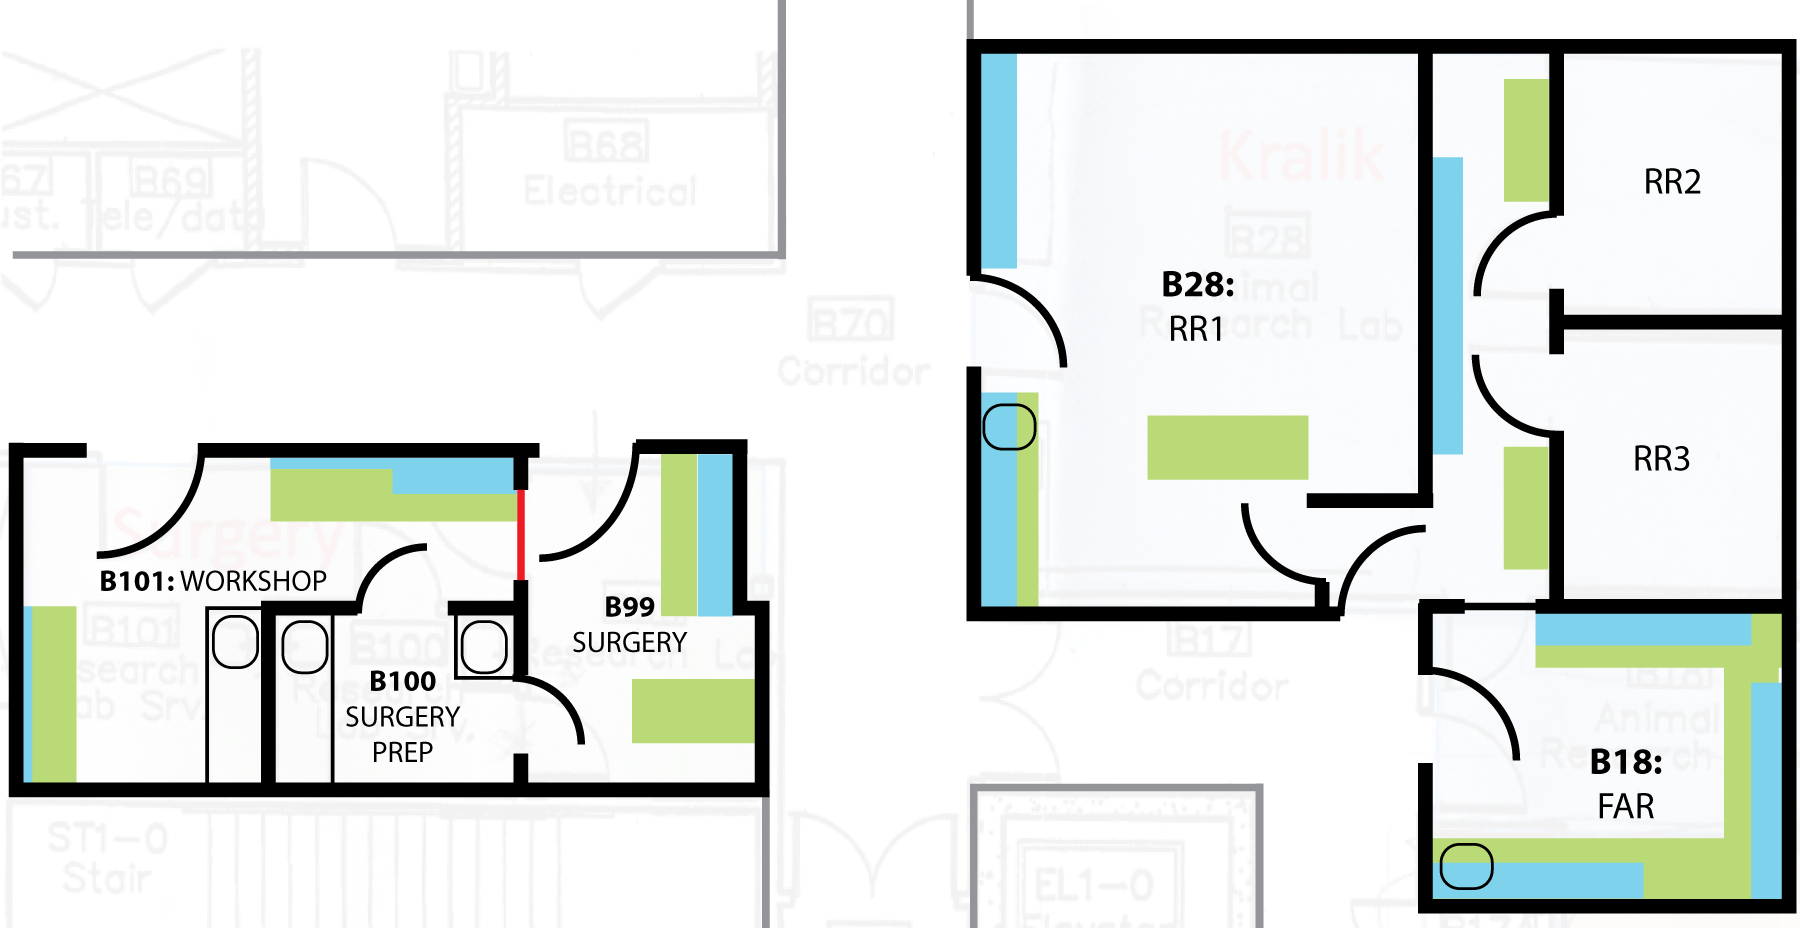
\includegraphics[width=\linewidth]{images/MvdM_labmap.png}
}
\caption{Map of the lab, in the Moore basement.}
\label{fig:labmap}
\end{figure}

\begin{itemize}
\item{{\bf Surgery}: a clean space for performing recovery surgeries
  on our animals. Currently also contains one of our head-fixed
  experimental setups for mice.}
\item{{\bf Surgery anteroom}: a staging area for surgery, containing
  consumables, surgical instruments, and the tools to keep everything clean.}
\item{{\bf Workshop}: a place to print, machine, build, and test
  things. Also contains spare stock for the surgery anteroom.}
\item{{\bf Fine Assembly Room (FAR)}: a clean space for the assembly
  and testing of brain implants. Contains microscopes, fine
  instruments, and extremely tiny parts.}
\item{{\bf Running rooms (1-3)}: spaces to run experiments.}
\end{itemize}

\section{General expectations}

In the lab, we assemble precision devices that will be surgically
implanted in live animals. We perform behavioral experiments that are
sensitive to changes in many different conditions. The amount of time
invested in these procedures, and the fact that we are doing this in
live animals, demand careful attention. In addition, lab space is
subject to general lab safety requirements (link) and IACUC
inspections (link).

The principle that guides the use of shared lab space is that any lab
member needs to be able to come in, find the items they need, and get
things done to a high standard. In addition, the condition in which te
lab spaces are kept should reflect pride taken in doing good work --
it will be seen and interpreted by others viewing our space.
Depending on the specific rooms this can mean somewhat different
things, discussed in more detail below, but there are some common
principles:

\begin{itemize}
\item{{\it Clean up after yourself}. Use common sense about when to do
  this. If you're in the middle of something and stepping out to get
  some lunch, it makes no sense to clear your work area. However, if
  you've finished what you were working on, definitely clean
  up. Before going home for the day is usually a good time to at least
  clean a bit. See the specific room schedules for more specific
  cleaning requirements.}
\item{{\it Organize where things are stored}. Any item in the lab has a
  home. Some individual items are sufficiently important that they
  have a dedicated place, such as ``final cut scissors''
  (PICTURE). Some items don't have a dedicated place but are a member
  of a more general category, such as ``BNC interconnects''. If you
  find an item that does not have an obvious home, check on Slack if
  anyone has suggestions, and/or create one for it. Creating a home
  for an item can be as simple as labeling a piece of a shelf
  somewhere. Make sure you tell everyone about it on Slack, in
  accordance with the Communication Principle!}
\item{{\it Track stock levels.} If something is running low, don't
  just ignore it. Post about it on Slack. Store parts that go with a
  certain piece equipment with that equipment (for instance, by taping
a ziploc baggie to it).}
\item{{\it Label things.} Any liquid and food containers MUST be labeled with
  the contents and expiry date, if applicable. When you open a new
  package of something, write on it when you opened it. When a new
  thing comes in, write on it when it was received.}
\item{{\it Treat tools with respect.} What may look like a cheap pair of
  scissors is likely to cost at least \$300. Use tools for their
  intended purpose, and use the correct tool for the job. For
  instance, don't use fine scissors to make rough cuts into hard
  materials. Don't use fine forceps to hold metal parts. \sidenote{Quick
  guide to forceps: ``\#55'' and ``\#5 Biologie'' are the finest.}}
\item{{\it Be safe.} The general lab safety training covers the
  basics, but specific spaces have hazards described below. First Aid
  kits are available in the FAR and in B101.}
\end{itemize} 


\section{Experiment rooms}

AKA ``running rooms''

These are the main spaces that our rats interact with. That has a few
consequences:

\begin{itemize}
\item{If you have a rat out, have the doors closed. Put a sign on the
  door saying, ``Experiment in Progress''.}
\item{Don't make changes to the layout of the room while you are
  running an experiment. Changing the cues and landmarks available can
  change what strategy animals use to solve a behavioral task.}
\item{Work to keep light levels, sound levels, and odor cues
  consistent.}
\item{Any surface rats interact with needs to be cleanable. So, no
  cardboard, unsealed wood, and so on.}
\item{Our IACUC protocols require cleaning apparatus at least weekly.}
\end{itemize}

Cleanliness and organization is important, but don't let that hold you
back in shaping your workspace to enable you do perform your
experiments well and efficiently. Tape procedures you are using to the
walls, print out the relevant atlas sections, make temporary storage
spaces for the tools you use frequently.

\section{Fine Assembly Room (FAR)}

The general directives about cleanliness and organization above all
apply. In addition, the following are important:

\begin{itemize}
\item{If you are working on something, it's okay to leave your work in
progress on work surfaces; however, please be considerate in how much
space you take up. Using a tray to hold you work is a great way to
limit your footprint, and to make it easy for others to use the space
if they need it.}
\item{Be particularly on guard for fragile items such as drives and
  silicon probes.}
\item{Close glass doors after you open them, and definitely when you
  leave for the day. They are there to protect sensitive equipment
  from dust and accidental touch.}
\end{itemize}

\section{Surgery and anteroom}

\newthought{Surgeries from which animals recover} demand that these
spaces are kept impeccably clean to minimize the risk of infection. In
addition, during surgery sometimes time is of the essence, and finding
what you are looking for quickly can make the difference between
success and failure. Thus, it is especially important that B99 and
B100 are organized well.

In particular:

\begin{itemize}
\item{Clean surfaces before and after surgery with Clidox
  (disinfectant) and then 70\% alcohol (solvent).}
\item{Treat the stereotax, pump, anesthesia trolley, and microscope
  with utmost care -- these are expensive, precision instruments.}
\item{Be on the lookout for low supply levels. For instance, after
  finishing a surgery, post to Slack if the oxygen cylinder has 1/4 or
  less left (there should always be a spare available in surgery).}
\end{itemize}

\section{Workshop}

Moore B101 contains several important tools:

\begin{itemize}
\item{Belt sander. Wear gloves and goggles when using it.}
\item{Rotary tool. Wear gloves and googles when using it.}
\item{3D printer.}
\end{itemize}

\section{Shared facilities}

Histology.

\section{Vivarium space}

Our rats are in Moore B63, and our mice in Moore B61.

Vivarium rooms need to have binders containing weights and animal records.

\section{Offices}

These are located on the ground floor of Moore, in the South wing
(graduate students) or in the West wing (lab techs and postdocs). The
grad offices house the lab library, consisting of books from MvdM's
personal library. Please ask MvdM before taking any book out of Moore,
and be vigilant about other labs borrowing but not returning them.

%%%%%%%%%%%%%%%%%%
%%%
%%%%%%%%%%%%%%%%%%
\chapter{Electronic resources}
\label{sec:elec-resources}

\section{GitHub}

GitHub hosts multiple repositories containing important lab
resources. These include:

\begin{itemize}

\item{\doccls{vandermeerlab}: the main lab codebase, containing MATLAB
  code for data input/output, preprocessing, data analysis, and
  visualization. Also includes a number of toolboxes created by others.}

\item{\doccls{mvdmlab-protocols}: contains descriptions of
  experimental procedures.}

\item{\doccls{mvdmlab-tasks}: contains descriptions of behavioral tasks.}

\item{\doccls{mvdmlab-management}}: hosts project boards and issues
  for lab admin, most importantly the
  \href{https://github.com/vandermeerlab/mvdmlab-management/projects/1}{ordering
    board}.

\item{\doccls{mvdmlab-designs}: contains CAD designs for use with our
  3D printer or printing services.}

\item{\doccls{papers}: code and data associated with the lab's publications.}

\item{Assorted project-specific repositories.}

\end{itemize}

To access some of these repositories, you need to be a member of the
\href{www.github.com/vandermeerlab}{vandermeerlab organization}. Ask
MvdM to become a member. Although you can view files on the
repositories through the GitHub website, you'll need to learn how to
use \href{https://www.codecademy.com/learn/learn-git}{git} in order to
use code stored there, and to contribute.

\section{Slack}

\href{Slack}{www.slack.com} is a software platform for having group
conversations in topic-specific channels. The lab Slack is
\url{mvdmlab.slack.com}. If you are joining the lab but haven't
received an invite yet, please let MvdM know.

\begin{marginfigure}%
  
\includegraphics[width=\linewidth]{images/slack.png}
  \caption{Slack.}
  \label{fig:slack}
\end{marginfigure}

The lab Slack is used for everyday communication about all aspects of
the lab's work, ranging from animal-related logistics and ordering
supplies to logging and discussing ongoing project results and sharing
grants. I suggest you join all channels initially -- even channels on
topics not necessarily related to your interests you should look at on
occasion to see what is happening.

\section{Wiki}

The lab \href{http://discovery.dartmouth.edu/~mvdm/wiki/}{wiki}
contains data analysis tutorials and other resources.

\section{Calendar}

The lab has a Google account (username \doccls{mvdmlab}, password
\doccls{ozomatl1}) which is associated with a number of calendars. All
experiment rooms and surgery have their own calendar, which you should
use to schedule your planned use of these rooms. The main lab calendar
contains labmeeting times, other scheduled events (e.g.\ journal
clubs), and times different lab members will be away.

\section{Mailing list}

The lab mailing list is used for announcements such as lab meetings
and journal clubs. If you are joining the lab, MvdM will sign you up.

\section{Lab server}

The lab server, physically located in MvdM's office, is the local
storage point for all the lab's data. Information on how to access it
can be found in the \#server channel on Slack. It contains a number of
folders, most importantly:

\begin{itemize}
\item{{\bf Promoted}: data folders that have been
  preprocessed\sidenote{See section XXX for an explanation of what
    data preprocessing enatils.} and can be used for data analysis.}
\item{{\bf InProcess}: data that is in the process of being promoted.}
\item{{\bf Incoming}: raw data. After acquiring data in an experiment,
  make sure to upload the data to the server; see the Computing
  section for details.}
\item{{\bf Tutorials}: example data sessions used for data analysis
  tutorials.}
\item{{\bf Dropoff}: a temporary folder that can be used for sharing
  files across the lab.}
\end{itemize}

\section{Others}

We use Dropbox\sidenote{Credentials are \url{mvdmlab@gmail.com}$/${\tt
    ozomatl1}.} to facilitate sharing of files across computers. It
should never be used for storage of data! If you see an opportunity to
promote any files currently on Dropbox to the relevant GitHub repo,
please do so (or create an issue first).

%%%%%%%%%%%%%%%%%
%%% COMPUTING %%%
%%%%%%%%%%%%%%%%%
\chapter{Computing}

\newthought{Computing plays an increasingly important role} in
(neuro)science and is central to many aspects of the lab's
workflow. The safety of your hard-won data, the integrity and
reproducibility of your analyses and results, the ongoing development
and sharing of the best protocols and procedures, and the speed with
which you can accomplish your goals all depend critically on correct
use of the lab's computing resources.

Because many of these are shared (experimental machines) and/or
inherently collaborative (lab database, codebase) it is especially
important to be aware of the issues below. Experience with some of the
more advanced concepts and tools is a highly valued skill in many labs
and workplaces; mastery of these will set you apart from many of your
peers.

\section{Lab computers}

The lab's computers are a mixture of custom builds (assembled from
parts by MvdM or someone else brave enough!), designed for a
particular role, and general-purpose workstations purchased from
Dartmouth Computing Services. The different roles determine the best
way to use each machine. The roles are:

\begin{itemize}
\item{Single-user machines in offices, one for each grad
student/tech/postdoc.}
\item{Shared machines. There is one in the FAR (B28), for use with the
  NanoZ and high-power microscope; one in B101, for use with the 3D
  printer; a laptop in surgery; and one computer associated with each
  data acquisition system (Neuralynx, Open Ephys).}
\end{itemize}

\subsection{Single user machines}

One of these will be exclusively yours to use during your tenure in
the lab. You are free to install software and change settings to suit
your needs as long as any changes (1) do not interfere with the
machine's ability to support research, and (2) fall within the
Dartmouth Computing guidelines\sidenote{link}. However, remember that
this is still a lab (Dartmouth)-owned machine, and should not be
extensively used for private activity. You can feel free to choose
your own username and password credentials.

Single user machines have a boot drive (C:) for the operating system
and frequently used software. This is a fast SSD drive with limited
space, so be mindful of what you install here. Absolutely do not use
this drive for any documents or data; use the data drive (D:) for this.

Many single-user machines use a RAID (automatically ``mirrored'')
storage array for the D: drive.  This means that if one hard drive
fails, the data is still available on the other.  However, mirroring
will not help you if you accidentally delete or overwrite files. For
this reason, {\it data} should always be available on the lab server,
{\it code} should be regularly pushed to GitHub and/or stored on
Dropbox\sidenote{...or a similar service such as Google Drive; note
  that Dropbox has a free academic account upgrade.}, and {\it
  documents} (e.g.\ your grant application, paper, or thesis) should
be on Dropbox or equivalent.

If you see Windows updates to install on any machine, go ahead and
install them. If a computer needs rebooting because of updates and you
can do so safely, go ahead.

\subsection{Shared machines}

Unlike the single user machines, when using the shared machine you
will need to consider how your actions affect other users. A few
guidelines:

\begin{itemize}
\item{If need to save your work, create a folder with your name on the
  Data (D:) drive. Do not leave work or data files on the desktop. If
  you find anything that's not supposed to be there on the desktop or
  anywhere else, put it in the lost-and-found folder on the desktop.}
\item{Do not install any software, or change any software and system
  settings, without discussing with MvdM first. Do not delete any
  files, but place them in the lost-and-found folder on the Desktop
  instead.}
\item{If you log in to web services, consider logging out when you
  are done.}
\end{itemize}

\subsection{Experimental machines}

The above considerations for shared machines apply. In addition:

\begin{itemize}
\item{If you acquire data for your project, use correct renaming and
  backup procedure when you finish your acquisition session. This is
  absolutely essential: data is expensive, and you individually and
  the lab as a whole cannot afford to lose any of it, EVER. Do not
  leave data in the acquisition folder.}
\item{If you encounter a potential data file or folder that is not
  yours and seems lost, make an effort to find out whose data it might
  be.}
\item{NEVER delete anything that looks like it might be data, unless
  you are absolutely certain that it has been backed up correctly.}
\end{itemize}


\section{Printing}

The departmental printer (in XX) is the primary way to print
stuff. Please be considerate when using the printer. Keeping an
electronic library of PDFs using an iPad, Dropbox and iAnnotate is a
worthwhile investment that will make it much easier to find papers and
your comments in the future, and will save a LOT of paper!

We also have a lab printer in the FAR. Only use this printer for
printing experiment-related documents such as animal weight sheets and
protocols.

\section{Skills}

To be written.

Basic skills: learning about your filesystem, what makes sense to
store where. Learn to use the command line.

Learn to code. MATLAB and Python are the most important. In our
subfield of neuroscience, MATLAB is still the most used, but Python is
gaining ground.

Good coding practices; style guides.

How to ask good questions. Stack Overflow on how to create a
\href{https://stackoverflow.com/help/mcve}{minimal, complete, and
  verifiable} example.

\section{Software}

In general, you should feel free use whatever software is the best
tool for the job\sidenote{...where ``best'' is defined as the
  intersection between the capabilities of the software itself,
  suitability for the task at hand, and the user's ability to use it
  correctly.}, and you should feel free to do so. However, there are
startup costs associated with learning how to use new software, and
the lab has built up expertise and resources in a number of software
packages that work well. Learning to use these software packages will
help you be productive in the lab, and will be applicable in other
settings as well.

\begin{marginfigure}
\centering{
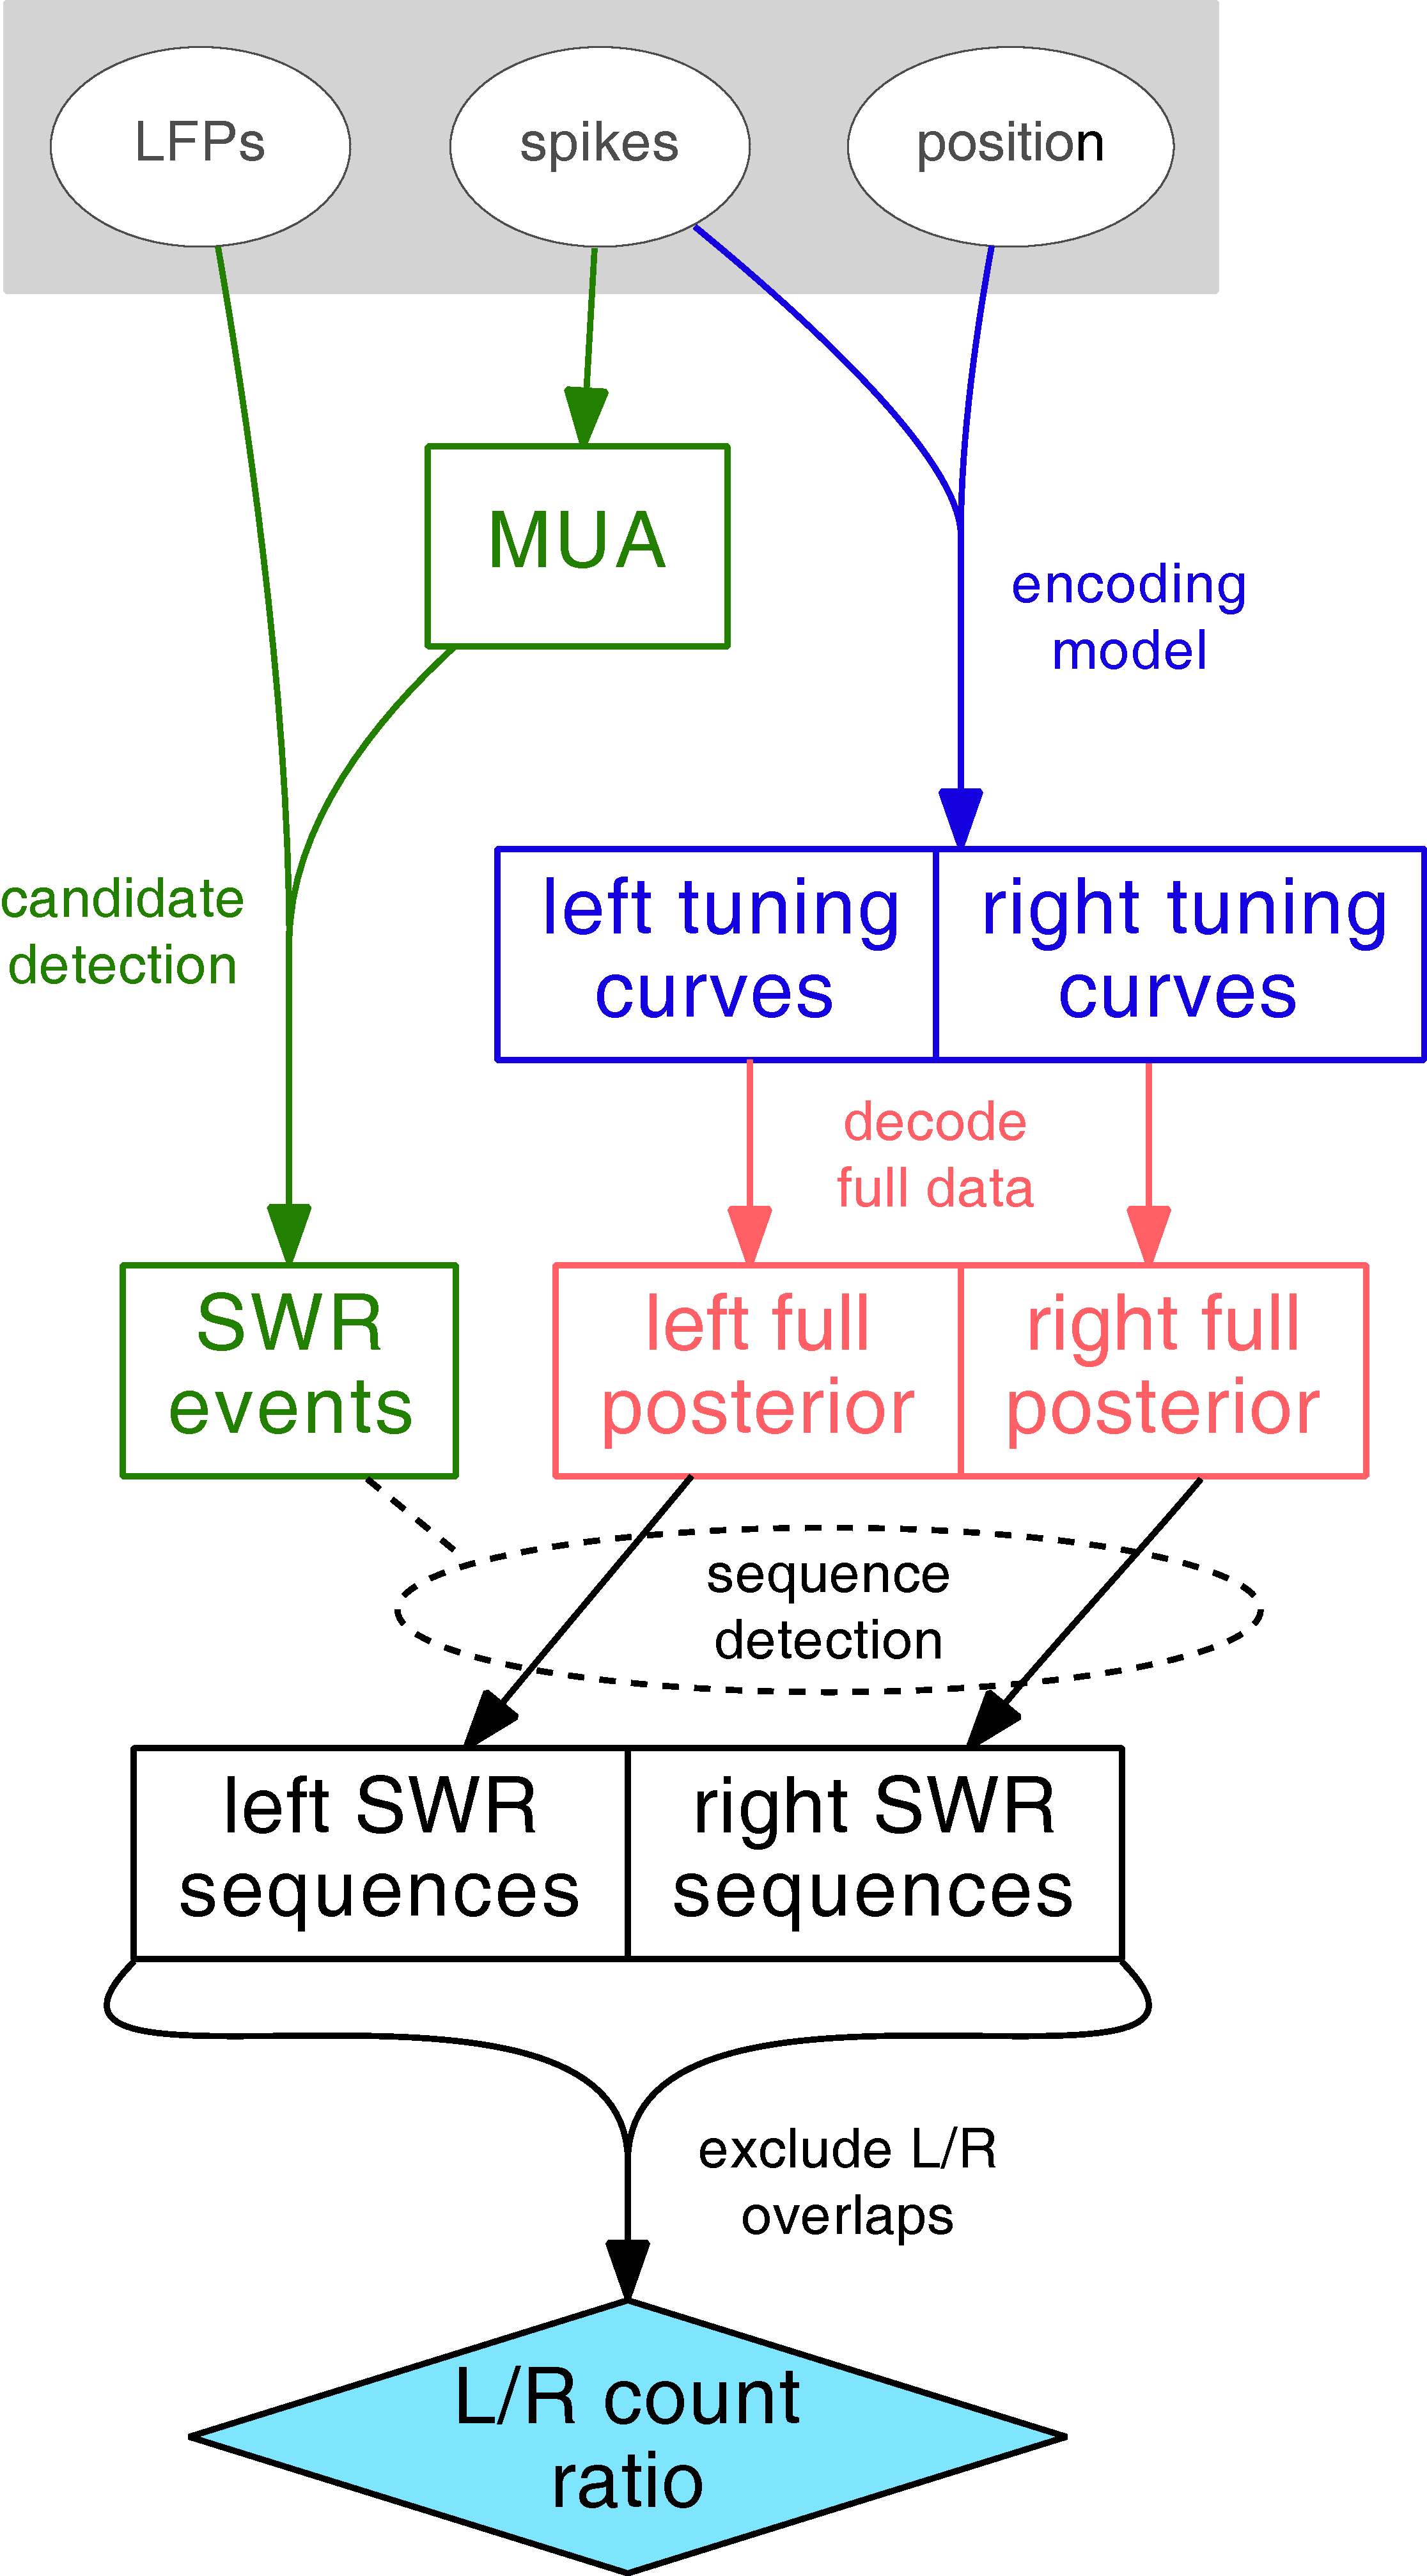
\includegraphics[width=\linewidth]{images/analysis_schematics.pdf}
}
\caption{Example data analysis workflow, made with \href{www.graphviz.org}{Graphviz}}
\label{fig:analysis-schematic}
\end{marginfigure}

\begin{itemize}
\item{{\bf Git} is a tool for ``collaborative version control'': a way
  to keep track of changes made to files such as computer code,
  experimental protocols or manuscrupt drafts, and to coordinate those
  changes across multiple contributors.}
\item{{\bf MATLAB} is a scientific computing environment that includes
  a programming language, libraries for performing specific tasks, a
  development environment with a fully featured editor, debugger, and
  interpreter, and many other features. It is widely used for data
  analysis in neuroscience. Although it is not free, Dartmouth has a
  site license that enables you to use it
  (\href{http://caligari.dartmouth.edu/downloads/matlab}{download
    page}). Python is becoming increasingly popular, and is far more
  widely used than MATLAB outside neuroscience. However, various
  toolboxes used in the lab such as Chronux and FieldTrip are still
  MATLAB-only, and MvdM is still a beginner in Python.}
\item{{\bf Adobe Creative Suite} is expensive, but produces superior
  documents. We use Illustrator to touch up and group together figure
  panels for manuscripts based on raw output from MATLAB or Graphviz,
  and to make posters. Photoshop is sometimes used to process image
  files such as those from histology. Free alternatives such as
  Inkscape and GIMP exist, can do the job for simple documents, but I
  don't (yet) recommend them for publication-quality output.}
\item{{\bf Graphviz} produces schematics such as the one in Figure
  \ref{fig:analysis-schematic}. Unlike
  `what-you-see-is-what-you-get'' design software such as Photoshop
  and Illustrator, the Graphviz tools create graphics from a plain
  text source file. The source file contains a recipe for what the
  graphic output should look like.}
\item{\LaTeX. Unlike ``what-you-see-is-what-you-get'' content creation
  programs such as Word, LaTeX creates documents from a plain text
  source file. The source file contains instructions for what the
  document should look like. Compared to Word, LaTeX does much better
  with equations, produces more professional-looking
  documents\sidenote{Especially where typesetting features such as
    spacing, kerning, and ligatures are concerned.}, and makes it much
  easier to maintain large documents.}
\end{itemize}

Note that several of these require you to use the Command Line
(Terminal).

\subsection{Operating Systems}

Lab computers use Windows and/or Ubuntu Linux. There are a few reasons
for this: the data acquisition machines require Windows (Neuralynx) or
Windows/Linux (Open Ephys), and custom machine builds are generally
cheaper for PCs than for Apple Macs. Nevertheless, many lab members
have Mac personal laptops that run OS X, and most of the above
software works fine on them. However, some Neuralynx loaders only work
on Windows, some codebase functions have only been compiled to work on
some OSes, and the lab only has licenses for some software (Adobe) to
work on Windows.

%%%%%%%%%%%%%%%%%%%%%%%%%
%%%% DATA MANAGEMENT %%%%
%%%%%%%%%%%%%%%%%%%%%%%%%
\chapter{Data management}

\newthought{Data is valuable.} After taking into account the number of
hours that went into training an animal, building a hyperdrive,
preparing for and performing surgery, painstakingly turning
electrodes; animal housing costs, costs of parts and consumables, and
so on, the cost of a single subject worth of data can run into tens of
thousands of dollars -- and this is without the moral calculation of
considering an animal's life. Data therefore needs to be treated with
the greatest respect: specifically, it needs to be managed so that it
can be maximally useful. The {\it first requirement} of data
management is that data needs to be available -- i.e.\ backed up so
that it can never be lost, and accessible by those who need it. Our
lab is committed to \doccls{Open Science}, of which public data
sharing is one component. Increasingly, journals and funders demand
that data is made publicly available. The {\it second requirement} of
data management is that the data needs to be organized such that it
can be easily understood and used.

Before discussing how these two requirements -- data storage and data
organization -- are implemented in the lab, it is useful to
distinguish between different categories of data.

\begin{itemize}

\item{{\bf Raw data} is what gets saved on a data acquisition machine,
  such as a running room computer connected to a Neuralynx recording
  system, or a machine connected to a microscope. Depending on the
  data you collect, a single session may yield many different files,
  such as behavioral tracking data and neural recording data, or a
  single file (an image). Raw data is only rarely suitable for
  analysis beyond a few quick checks. At a minimum, freshly acquired
  data sets typically must be annotated, and/or the files
  systematically renamed -- for instance, with the ID of the
  experimental subject and some information about recording locations
  -- so that the analyst can select which files to analyze, and combine
  results across sessions and subjects. More complex pre-processing
  steps include spike sorting (the process of assigning spike
  waveforms to putative single neurons to obtain their spike times),
  artefact removal, and many others.}

\item{{\bf Promoted data} is data that is ready for analysis. Data
  files need to be organized in a specific folder structure, named
  according to the naming scheme, and supplied with annotations
  describing the data. If applicable, various preprocessing steps may
  have been carried out, for instance spike-sorting of raw voltage
  traces into spike trains of putative single neurons, filtering
  of position data to remove artifacts, and definition of trials on a
  behavioral tasks. PDFs of handwritten notes and procedure logs, and
  images of histology may also be included. A promoted data set
  typically does not include the raw data. Promoted data should be
  sufficiently well described and organized such that a competent
  reviewer or collaborator can use it.}

\item{{\bf InProcess data} is data that is being worked on to move it
  from \doccls{raw} to \doccls{Promoted}.}

\end{itemize}

\section{Data storage}

\newthought{Immediately after data is first acquired}, do the
following:

\begin{itemize}
\item{Create and/or rename the new data folder according to the
  \doccls{Lab Data Naming Scheme}.}
\item{If applicable, compress any files that are large and
  compressible: typical examples include Neuralynx .nvt (video
  tracking) files\sidenote{See section XXX for a quick primer on data
    compression.}.}
\item{Upload the data to the {\it Incoming} folder on the lab
  server. See section XXX for instructions.}
\item{Move the data out of the location where it is saved, into a
  folder specific to your subject or experiment.}
\item{Following completion of data collection from that subject or
  experiment, verify that indeed all data is correct and present on
  the server, and then delete it from the data acquisition
  machine.\sidenote{This is an important step, because if there is no
    space available on a data acquisition machine, we cannot acquire
    more data!}}
\end{itemize}

The lab server uses a redundant data storage system that can tolerate
failure of a single hard drive without causing loss of data. The
contents of the datavault folder are periodically backed up to
``cold'' offsite storage. However, it is good practive to also make
your own personal backup of your raw and promoted data. One good way
of doing this is to store that data on your desktop workstation, or
move it to an external HDD, just in case.

\section{Data promotion}

What exactly is included in a promoted data set depends on the
specific experiment, but typical features include the following:

\begin{itemize}
\item{Data should be organized and (re)named according to the lab Data
File Naming Scheme (link).}
\item{Make sure raw and intermediate data files that are no longer
  needed are removed.}
\item{\doccls{ExpKeys} file.}
\item{If applicable, task-specific \doccls{metadata} file(s).}
\item{A description of the task/experiment.}
\item{PDFs of relevant task notes and histology.}
\end{itemize}

As you collect data, you should start drafting an example
\doccls{ExpKeys} file. Prior to starting data collection, you should
have created a \doccls{protocol} that describes the procedures
used. You should use this protocol as the basis for a description of
the task/experiment.

Examples of nice promoted data with description include Alyssa's
\doccls{MotivationalT} data (link) and Jimmie's \doccls{CueCoding}
data\sidenote{\url{https://github.com/jgmaz/vStrCueCoding}}.

\section{Data use cases}

Some examples (``use cases'') that motivate careful data management
include:

\begin{itemize}
\item{When analyzing your own data, you want to be able to easily
  specify which subject(s) and session(s) you are working on.}
\item{If you have a question that can be answered with someone else's
  data, you want to be able to ``plug in'' that data into your
  existing workflow. When I (MvdM) joined the Redish lab, I ran a
  comparison of dorsolateral striatum, ventral striatum, and
  hippocampus data\sidenote{van der Meer et al.\ Neuron 2010}. This
  was made possible through the use of a consistent data formatting
  and annotation scheme.}
\item{When publishing your work, it is the policy of the lab, and an
  increasing number of journals and funders, that your data is made
  publicly available. You want it to be easy to use and understand, so
  that your colleagues are not annoyed with you and you don't have to
  answer their emails telling you things aren't working.}  
\item{Before you get to publishing, you will need to convince MvdM
  of your results and conclusions. This likely invloves
  him running your code on your data. That will only work if you've
  organized your data correctly.}
\item{MvdM is always working on applications to obtain research
  funding. Some of these applications, and the pilot data used to
  support them, are planned in advance; others are more
  spur-of-the-moment, or even if planned, new insights can
  happen. Thus, there is often a need to produce an analysis or figure
  in short order. This is only possible, or at least made a lot
  easier, if the data is ready for analysis.}.
\end{itemize}

%%%%%%%%%%%%%%%%%%
%%% ONBOARDING %%%
%%%%%%%%%%%%%%%%%%
\chapter{Appendix: Onboarding}

If you are new to the lab, here is a list of items to get you started:

\section{Space and access}

\begin{itemize}
\item{Talk to MvdM to find out what desk space you can use. Feel free
  to customize the space to make yourself comfortable!}
\item{If you don't have a \doccls{campus ID card} (``DartCard'') yet, you can get one
from the
\href{https://www.dartmouth.edu/finance/employee-services/other_services/dartcard/}{office}
in McNutt. Once you have your card, go see Bess Ritter, the \href{https://pbs.dartmouth.edu/people?field_people_local_tags_tid=1916}{departmental
administrator} to introduce yourself, and get access.}
\item{While you're in the department office, say hi to Michelle Powers
and ask her for a key to your office.}
\end{itemize}

\section{Computing}

\begin{itemize}
\item{Get MvdM to add you to the \doccls{lab mailing list} and the lab
  \doccls{Slack}.}
\item{Slack MvdM your \doccls{GitHub username} so he can add you to the
  vandermeerlab organization.}
\item{Add the \doccls{mvdmlab calendar} to your inventory of calendars. See
  \hyperref[sec:elec-resources]{Electronic Resources} for details.}
\item{Install MATLAB on your computer if needed, and complete \href{https://rcweb.dartmouth.edu/~mvdm/wiki/doku.php?id=analysis:nsb2017:week1}{Module 1}
  of the lab's data analysis tutorials.}
\end{itemize}

\section{Training}

\begin{itemize}
\item{Get MvdM to add you to the lab's BioRAFT personnel list, so you
  will get invites to the relevant lab safety training.}
\item{Get MvdM to add you to the lab's animal protocol(s) so you will
  get invited to the on-line and in-person animal training.}
\item{Discuss your training goals with MvdM so you can start crafting
  a personalized Training Plan together.}
\item{Discuss making a Mentoring Agreement with MvdM.}
\end{itemize}

\backmatter

\bibliography{C:/Users/mvdm/Documents/library/LabManual}
\bibliographystyle{apa}


\printindex

\end{document}
